\documentclass{article}
\usepackage[utf8]{inputenc}
\usepackage[spanish]{babel}
\usepackage{listings}
\usepackage{graphicx}
\graphicspath{ {images/} }
\usepackage{cite}

\begin{document}

\begin{titlepage}
    \begin{center}
        \vspace*{1cm}
            
        \Huge
        \textbf{Proyecto Final}
            
        \vspace{0.5cm}
        \LARGE
        Ideas generales para el proyecto final Air-hockey 
            
        \vspace{1.5cm}
            
        \textbf{Carolina Jimenez Restrepo}\\
        \textbf   { c.c 1020470694}\\
        \textbf{Danier Santiago Ortega Restrepo}\\
        \textbf{c.c 1036681098 }
          \\  Grupo 3
            
            \vspace{2.9cm}
         
                   profesor: Augusto Enrique Salazar Jimenez
                   Curso: Informática II
        \vfill
            
        \vspace{0.8cm}
            
        \Large
        Despartamento de Ingeniería Electrónica y Telecomunicaciones\\
        Universidad de Antioquia\\
        Medellín\\
        Marzo de 2021
            
    \end{center}
\end{titlepage}

\tableofcontents
\newpage
\section{Sección introductoria}\label{intro}
¿Has jugado alguna vez al Air Hockey? Air Hockey es un juego bastante popular en los centros de juego y otros lugares donde la gente pasa el rato. No mucha gente tuvo la oportunidad de probarlo como un juego preinstalado en los sistemas operativos. El propósito del juego es golpear el disco a la portería del oponente con una paleta. El disco se coloca sobre una mesa especial, que produce un colchón de aire en la superficie de juego a través de pequeños orificios con el propósito de reducir la fricción y aumentar la velocidad de juego . El ganador es el jugador que anota 7 puntos primero. 
A continuacion presentaremos un conjunto de ideas y proyecciones para tener en cuenta en el proceso de desarrollo del proyecto final de Informatica II

\section{Ideas de realizacion}
\label{contenido}
\subsection{Idea principal}

El objetivo del proyecto es crear un juego para un solo jugador el cual jugara contra la maquina, al comenzar el juego aparecera la mesa o patio de juego y un menu con opciones.

\subsection{Diseño del juego}
Unas de las plataformas para el diseño serian: 

Tinkercad.com, en este entorno seria util para la creacion de graficos 2d o 3d para en la implementacion del proyecto.

\begin{figure}[h]
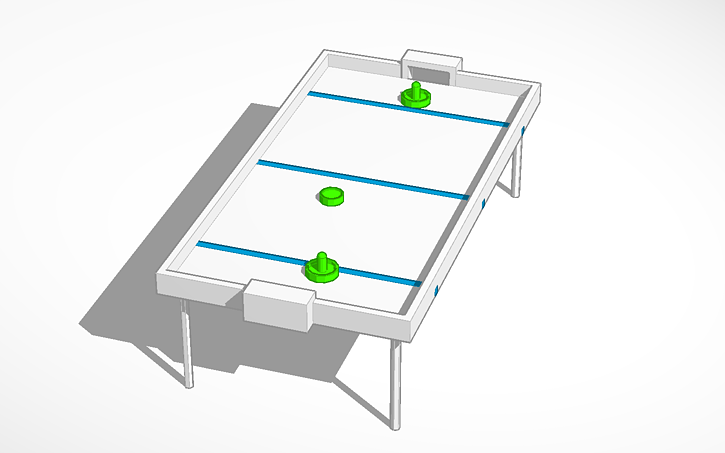
\includegraphics[width=5cm]{ideacion/plantilla_latex/imagenes/tinkercad_1.png}
\centering
\caption{imagen didactica}
\label{fig:cpplogo}
\end{figure}
La implementacion de un espacio fisico tri-dimensional o de dos dimensiones se tomara en cuenta a partir de la cantidad de memoria que se tenga a disposicion.


El juego constaria de unas partes las que son: mesa, barreras, porterias, puck(disco) y remos.

\section{ Imágenes de referencia} \label{imagenes}

En las Figuras (\ref{fig:Air-Hockey}), (\ref{fig:air-menu}), se   presentan imagenes de referencia que nos daran una idea más clara de como será el juego

\label{imagenes}
\begin{figure}[h]
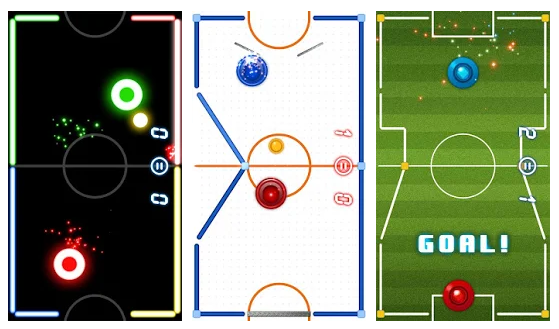
\includegraphics[width=5cm]{imagenes/Air-Hockey.png}
\centering
\caption{patio de juego}
\label{fig:Air-Hockey}
\end{figure}


\label{imagenes}
\begin{figure}[h]
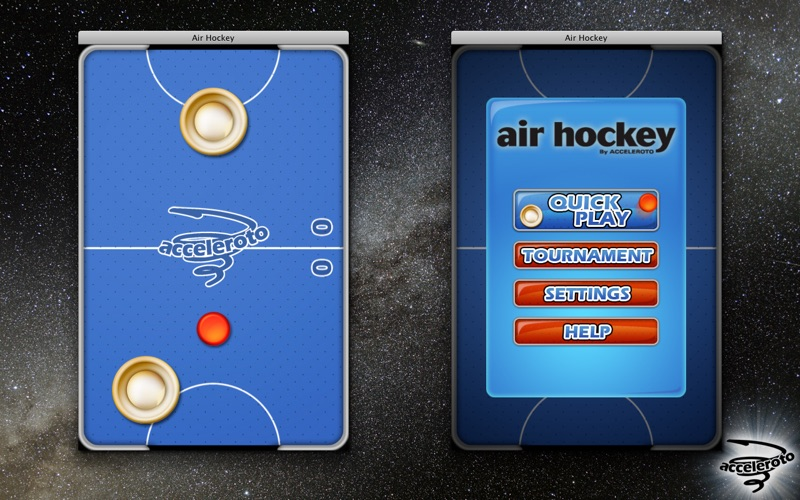
\includegraphics[width=5cm]{ideacion/plantilla_latex/imagenes/air-menu.jpg}
\centering
\caption{ menú}
\label{fig:air-menu}
\end{figure}

\end{document}
